\clearpage
\section{Phân hệ Giỏ hàng (Cart)}

\subsection{Đặc tả Use Case}
Phân hệ Giỏ hàng quản lý danh sách các món đồ uống mà khách hàng đã lựa chọn kèm theo các tùy biến cụ thể trước khi tiến hành tạo đơn hàng chính thức. Để tối ưu hóa tài nguyên máy chủ và mang lại phản hồi tức thì cho người dùng, phân hệ này được thiết kế theo kiến trúc lưu trữ phía máy khách (\textit{Client-side State Management}). Sơ đồ Use Case được minh họa tại Hình~\ref{fig:usecase-cart}.

\begin{figure}[H]
    \centering
    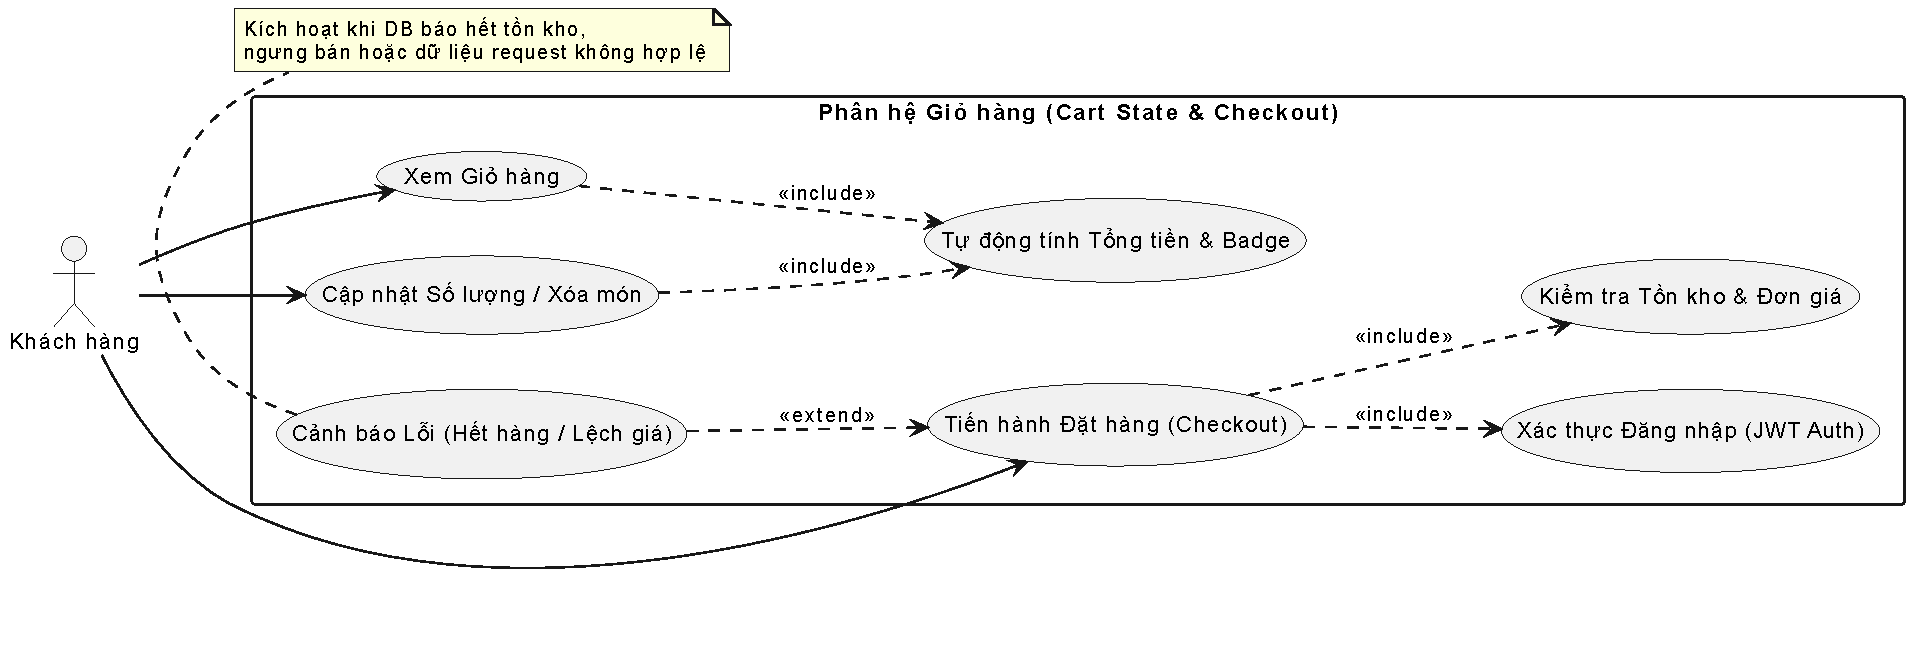
\includegraphics[width=0.75\textwidth]{figures/usecase-cart.pdf}
    \caption{Sơ đồ Use Case - Phân hệ Giỏ hàng}
    \label{fig:usecase-cart}
\end{figure}

\begin{table}[H]
\centering
\small
\caption{Đặc tả Use Case: Quản lý Giỏ hàng (UC-CART-01)}
\label{tab:uc-spec-cart}
\begin{tabularx}{\textwidth}{p{2.8cm}X}
\toprule
\textbf{Mục} & \textbf{Chi tiết Đặc tả} \\
\midrule
\textbf{Actor} & Khách vãng lai, Khách hàng đăng nhập \\
\midrule
\textbf{Tiền điều kiện} & Người dùng đã truy cập ứng dụng trên trình duyệt web. \\
\midrule
\textbf{Hậu điều kiện} & Danh sách món trong giỏ hàng, số lượng và tổng tiền tạm tính được cập nhật đồng bộ trong bộ nhớ máy khách (\texttt{localStorage} / Zustand state). \\
\midrule
\textbf{Luồng chính} & 
1. Người dùng thêm món từ trang chi tiết hoặc nhấn vào biểu tượng giỏ hàng tại thanh điều hướng (\texttt{Navbar}).\newline
2. Giao diện điều hướng sang trang \texttt{/cart}.\newline
3. Hệ thống nạp danh sách các món trong giỏ từ bộ nhớ cục bộ.\newline
4. Người dùng có thể tăng/giảm số lượng từng món, xóa từng món hoặc xóa toàn bộ giỏ.\newline
5. Bộ tính giá phía client tự động tính toán lại mục "Tạm tính" cho từng dòng và tổng giá trị đơn hàng.\newline
6. Khi người dùng nhấn "Thanh toán" (hoặc "Tiến hành đặt hàng"), hệ thống kiểm tra điều kiện đăng nhập trước khi chuyển sang bước đặt hàng. \\
\midrule
\textbf{Luồng ngoại lệ} & 
- Giỏ hàng không có sản phẩm nào: Giao diện hiển thị thông báo "Giỏ hàng của bạn đang trống" và nút điều hướng "Xem thực đơn". \\
\bottomrule
\end{tabularx}
\end{table}

\clearpage
\subsection{Sơ đồ Hoạt động (Activity Diagram)}
Quy trình quản lý thêm, sửa, xóa và tính toán giá trị giỏ hàng được thể hiện tại Hình~\ref{fig:activity-cart}.

\begin{figure}[H]
    \centering
    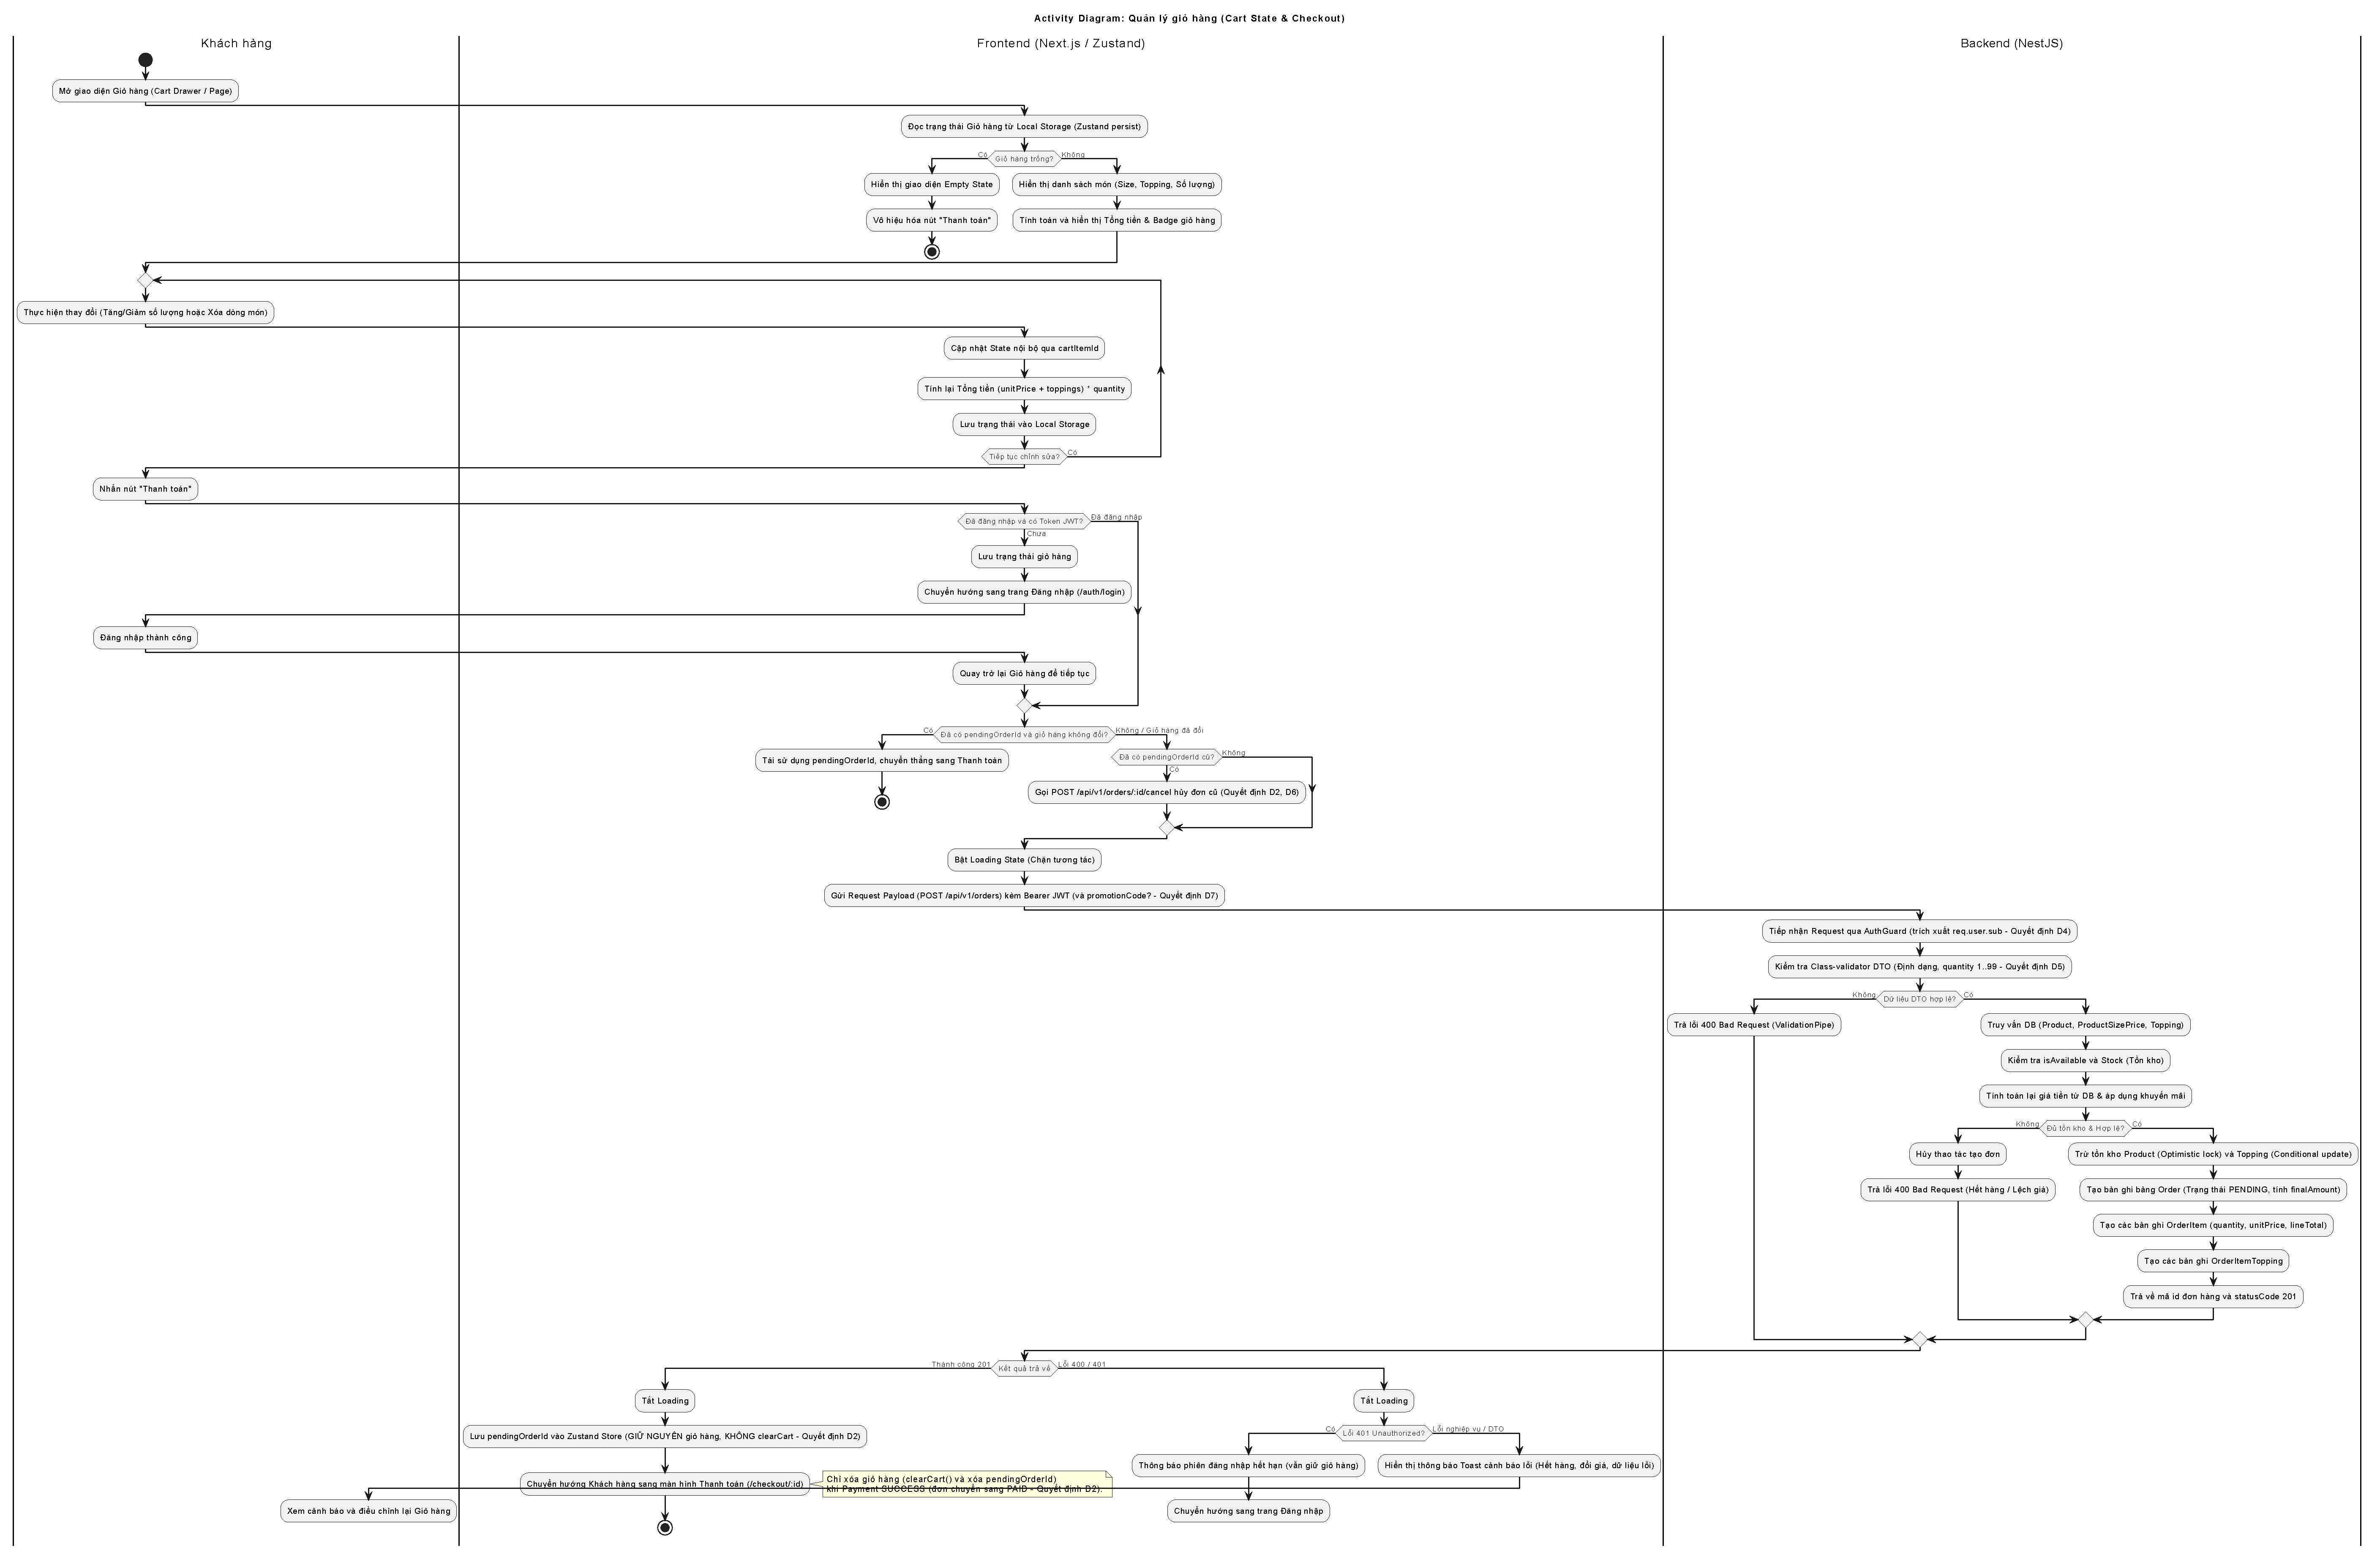
\includegraphics[width=\textwidth, height=0.80\textheight, keepaspectratio]{figures/activity-cart.pdf}
    \caption{Sơ đồ Hoạt động - Phân hệ Giỏ hàng}
    \label{fig:activity-cart}
\end{figure}

\clearpage
\subsection{Sơ đồ Tuần tự (Sequence Diagram)}
Sơ đồ Tuần tự minh họa luồng xử lý hoàn toàn khép kín ở phía Frontend giữa giao diện, Store quản lý trạng thái và LocalStorage tại Hình~\ref{fig:sequence-cart}.

\begin{figure}[H]
    \centering
    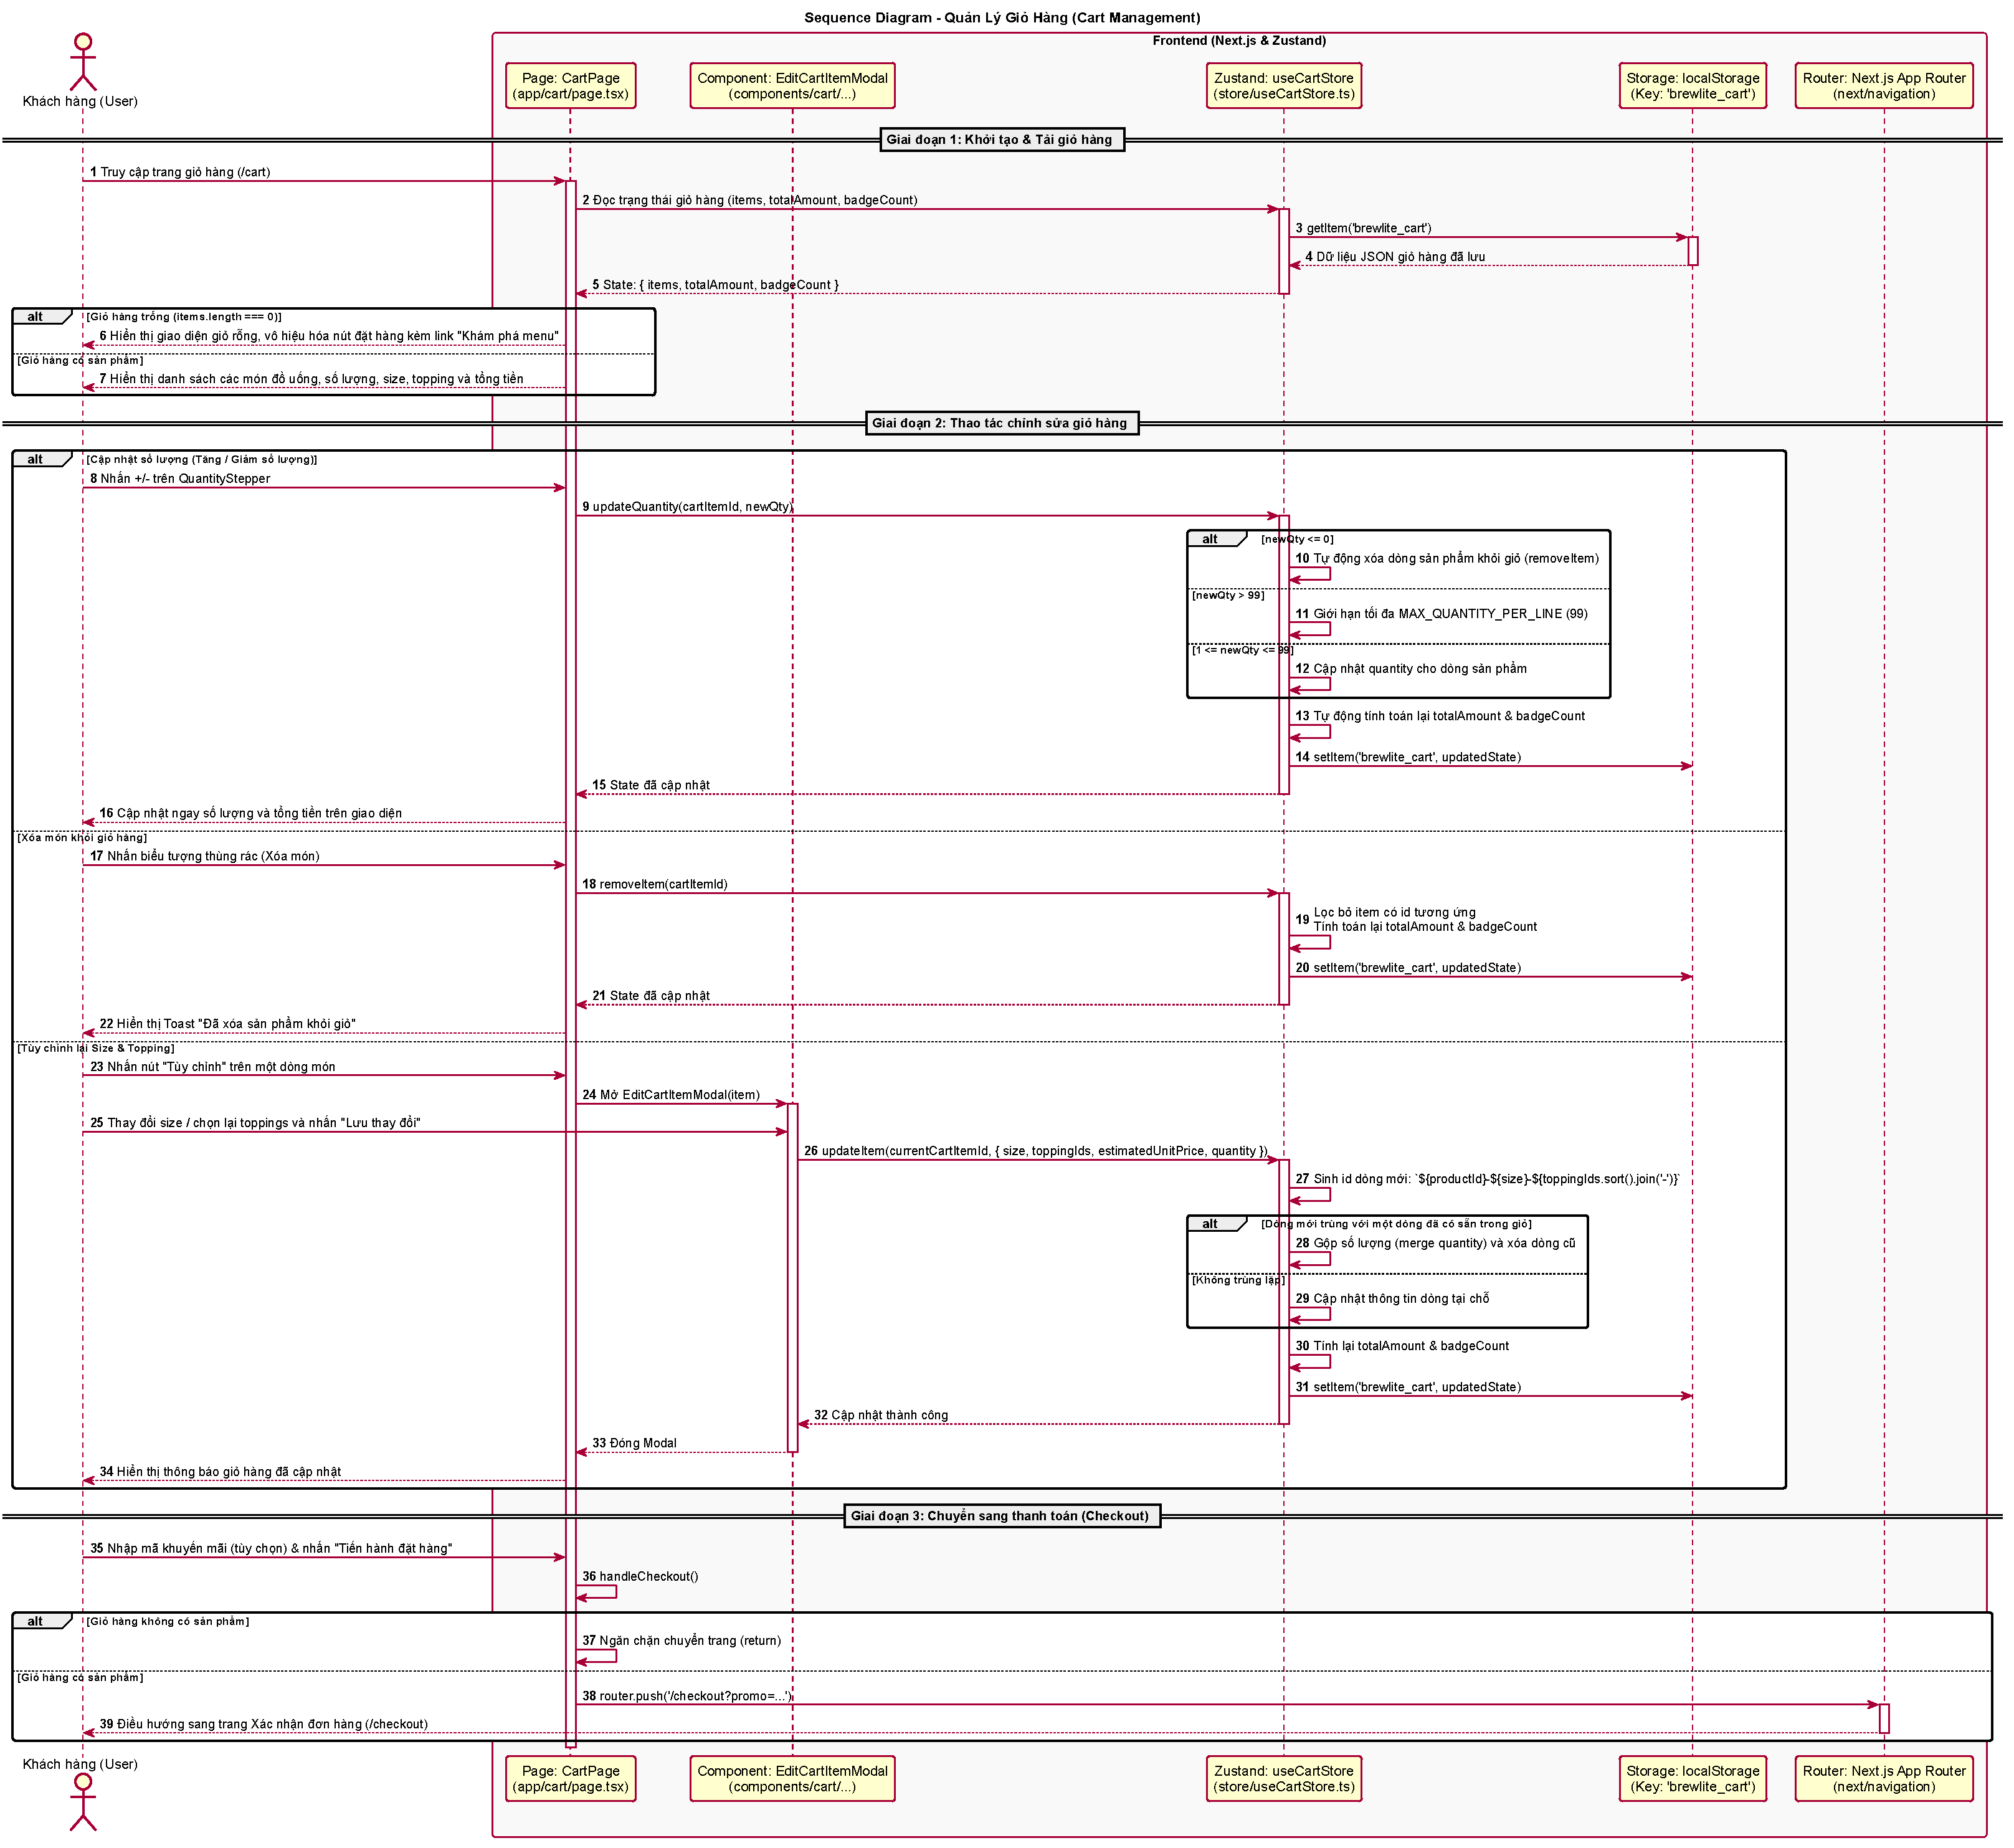
\includegraphics[width=\textwidth, height=0.80\textheight, keepaspectratio]{figures/sequence-cart.pdf}
    \caption{Sơ đồ Tuần tự - Phân hệ Giỏ hàng (Client-side Architecture)}
    \label{fig:sequence-cart}
\end{figure}

\clearpage
\subsection{Hợp đồng API và Ánh xạ Cơ sở dữ liệu}
\begin{itemize}
    \item \textbf{Đặc tính kỹ thuật (FE-Only):} Giỏ hàng trong BrewLite hoạt động hoàn toàn ở phía máy khách (\textit{Frontend-only}). Không có API endpoint riêng trên Backend và không tạo bản ghi trong cơ sở dữ liệu cho giỏ hàng tạm thời.
    \item \textbf{Cấu trúc đối tượng lưu trữ (\texttt{CartItem}):}
    Mỗi phần tử giỏ hàng được định danh bởi một khóa duy nhất sinh ra từ tổ hợp thuộc tính (\texttt{productId}, \texttt{size}, \texttt{sweetness}, \texttt{ice}, danh sách \texttt{toppings}):
    \begin{itemize}
        \item \texttt{id}: Mã duy nhất của món trong giỏ.
        \item \texttt{productId}: ID sản phẩm tham chiếu.
        \item \texttt{name}, \texttt{image}: Thông tin hiển thị.
        \item \texttt{size}, \texttt{sweetness}, \texttt{ice}: Các tùy biến đã chọn.
        \item \texttt{toppings}: Danh sách topping kèm giá đơn vị.
        \item \texttt{quantity}: Số lượng đặt (\(\ge 1\)).
        \item \texttt{unitPrice}: Đơn giá đã bao gồm phụ thu kích cỡ.
        \item \texttt{subtotal}: Tổng tiền của dòng món = \((unitPrice + \sum toppingPrice) \times quantity\).
    \end{itemize}
\end{itemize}

\subsection{Kịch bản Kiểm thử (Test Cases)}
\begin{table}[H]
\centering
\small
\caption{Tóm lược các Ca kiểm thử tiêu biểu - Phân hệ Giỏ hàng}
\label{tab:tc-cart}
\begin{tabularx}{\textwidth}{llp{2.6cm}p{3cm}Xc}
\toprule
\textbf{Mã TC} & \textbf{Loại} & \textbf{Tiền điều kiện} & \textbf{Endpoint / Màn hình} & \textbf{Kết quả mong đợi} & \textbf{Trạng thái} \\
\midrule
\texttt{TC-CART-UI-01} & Giao diện & Giỏ chưa có món & Màn hình \texttt{/cart} & Hiển thị thông báo giỏ hàng trống & Chưa chạy \\
\texttt{TC-CART-UI-02} & Nghiệp vụ & Đã thêm 1 món & Màn hình \texttt{/cart} & Hiển thị đúng tên, size, mức đường, đá, topping & Chưa chạy \\
\texttt{TC-CART-UI-03} & Nghiệp vụ & Đang có món & Nút tăng/giảm & Cập nhật số lượng và tự động tính lại tổng tiền & Chưa chạy \\
\texttt{TC-CART-UI-04} & Nghiệp vụ & Đang có món & Nút xóa món & Món bị loại bỏ khỏi danh sách, tính lại tiền & Chưa chạy \\
\bottomrule
\end{tabularx}
\end{table}

\subsection{Giao diện Người dùng}
\begin{figure}[H]
    \centering
    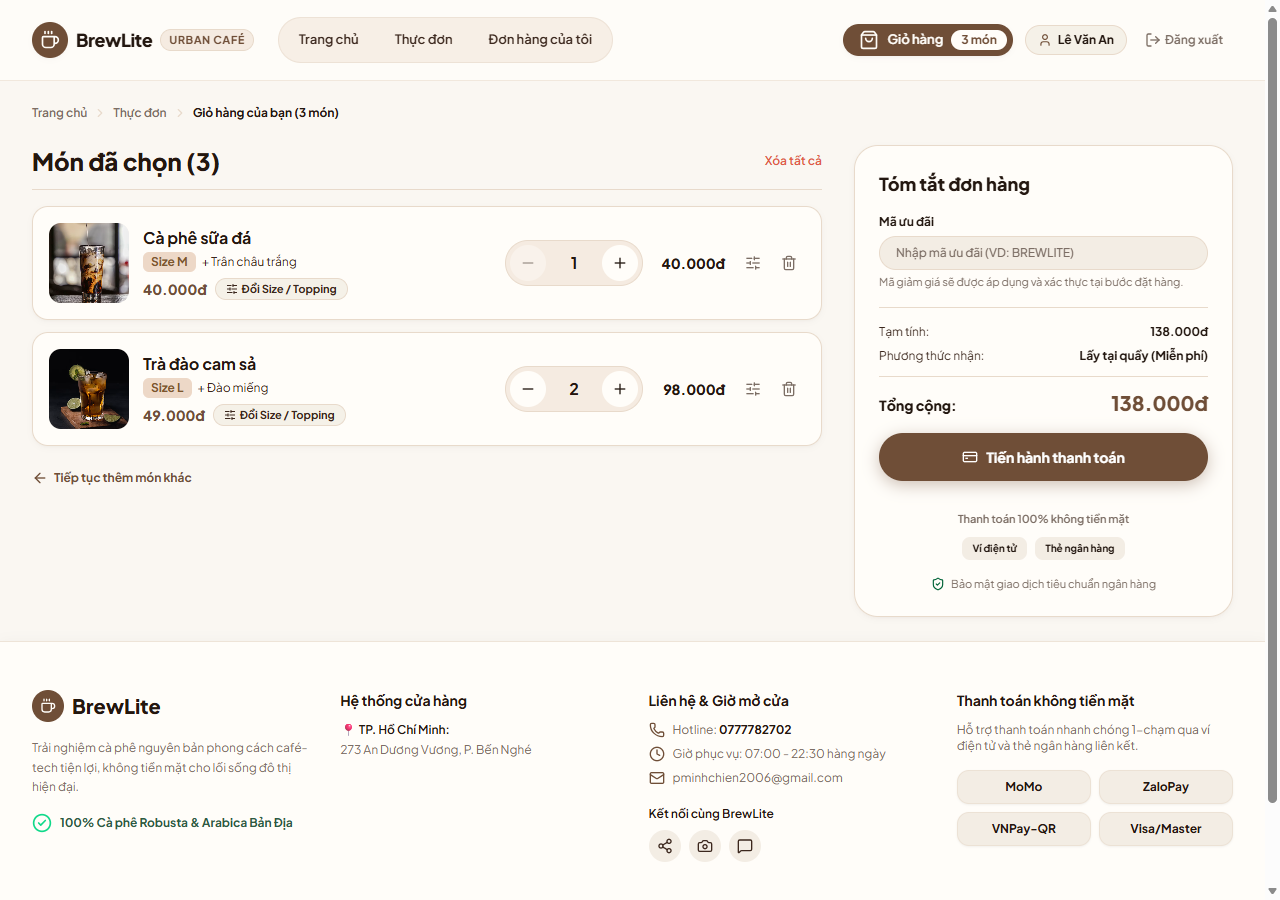
\includegraphics[width=0.92\textwidth]{figures/ui-cart.png}
    \caption{Giao diện Quản lý Giỏ hàng và Điều chỉnh số lượng BrewLite}
    \label{fig:ui-cart}
\end{figure}
